\subsection{Clustering}
L’idée est d’écarter les items (resp. les utilisateurs) jugés non représentatifs pour un utilisateur (resp. item) donné. On réduit ainsi la dimension de la matrice tout en minimisant la perte de données avant d’effectuer les calculs de recommandation.
Pour ce faire, on utilise des méthodes de partitionnement qui consistent à regrouper les éléments similaires. La méthode la plus connue est k-means.\par
Un cluster est un regroupement d'éléments qui sont similaires entre eux et dissimilaires aux autres éléments appartenant aux autres cluster. Le but de l'algorithme k-means est donc de créer k clusters à partir d'un ensemble d'utilisateurs.

\begin{figure}[H]
	\begin{center}
		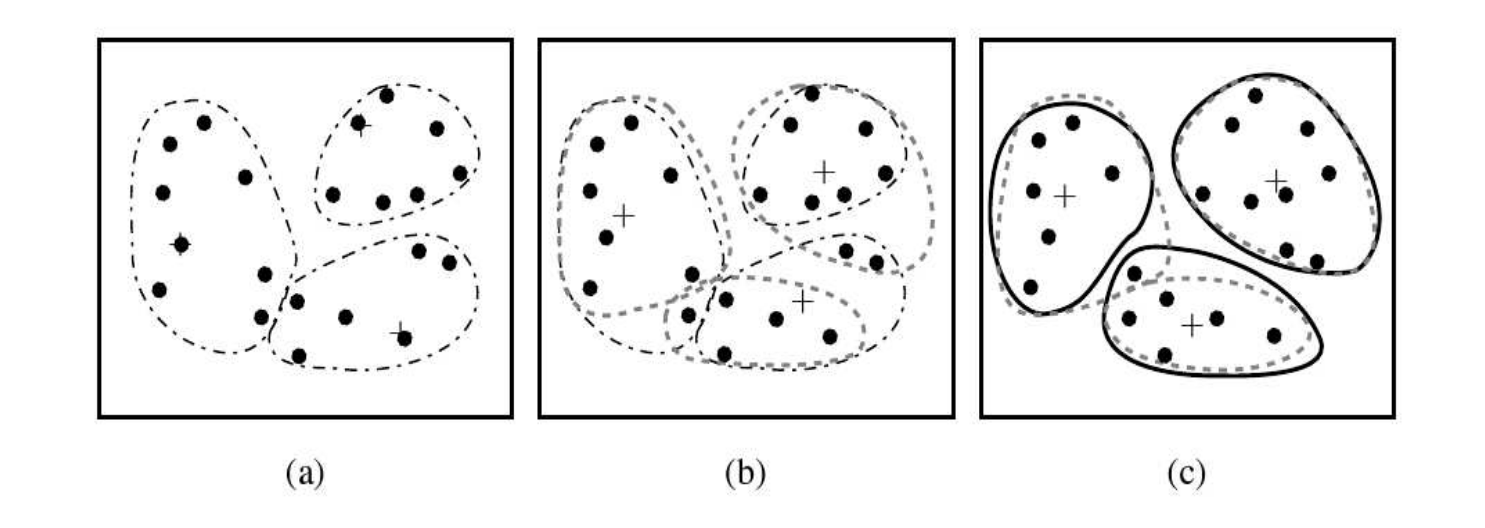
\includegraphics[scale=0.27]{img/k_means.png}
	\end{center}
	\caption{Illustration de l'algorithme k-means pour k=3}
\end{figure}
\newpage
Le fonctionnement de cet algorithme est le suivant :
\begin{algorithm}
\caption{Algorithme de partitionnement k-means}
\textbf{INPUT:} k : nombre de clusters, U : l'ensemble des utilisateurs\\
\textbf{OUTPUT:} k clusters
\begin{algorithmic}
\STATE Choisir aléatoirement k centroïdes initiaux de clusters
\REPEAT
\STATE Réaffecter chaque utilisateur de U au cluster dont il est le plus similaire
\STATE Recalculer les distances des utilisateurs dans chaque cluster
\STATE Mettre à jour les centroïdes
\UNTIL{Stabilité des centroïdes}
\end{algorithmic}
\end{algorithm}

Cet algorithme présente comme avantage la facilité de mise en oeuvre ainsi que son efficience. De plus, si on prend un groupe de n utilisateurs et que l'on souhaite réaliser k clusters en t itérations, la complexité de l'algorithme est en $\Theta(knt)$.\par
En revanche, l'algorithme est très sensible aux données aberrantes. En effet, un utilisateur très éloigné de tous les autres sera tout de même intégré à un cluster et affectera son centroïde.\par
Il existe un autre algorithme qui est moins sensible à ce type de données : le "PAM" pour Partionning Around Medoïds ou encore k-medoïde. Sans rentrer dans les détails, cet algorithme ressemble au k-means à la différence qu'il prend un utilisateur comme centroïde du cluster (qui est alors appelé médoïde).
Néanmoins, cet algorithme a une complexité plus élevée, en $\Theta(tk(n-k)^2)$. C'est pourquoi il est moins utilisé que k-means.
